\chapter{Parallel Computing Alternatives}
\section{Parallel Virtual Machine}
PVM is based on a dynamic computing model, where nodes can be added/deleted on the fly and parallel tasks can be spawned/killed during the computation. This provides fault tolerance and adaptability, but it is not as rich in message passing features as MPI. However, as it is a virtual machine, it provides features ideal for creating dynamic parallel programs.

Each host participating in the virtual machine executes the \texttt{pvmd} daemon. The \texttt{pvmd}s of all the hosts combine to form the virtual machine. Applications with PVM primitives can contact their local \texttt{pvmd} to interact and/or execute actions across the virtual machine. This is shown in \autoref{fig:screenshot063}.

\begin{figure}
\centering
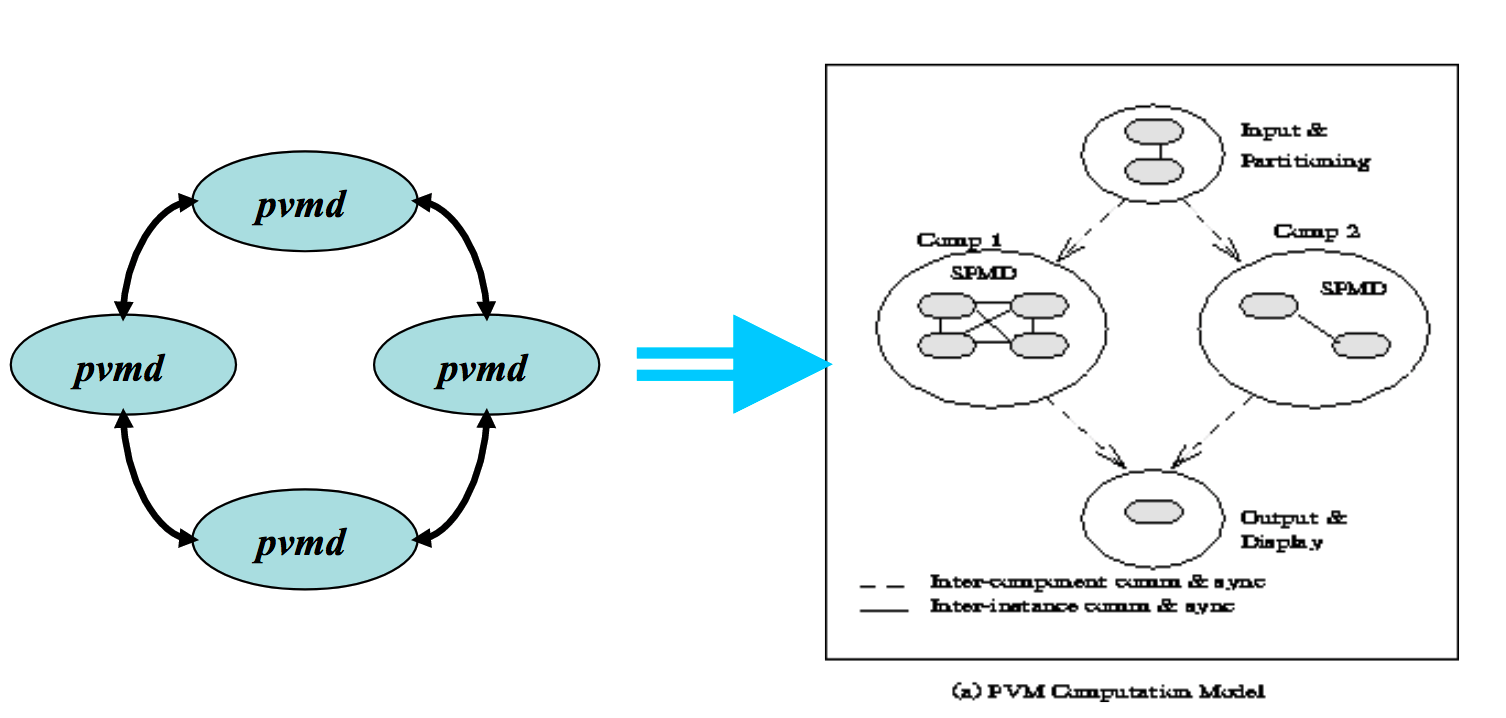
\includegraphics[width=0.7\linewidth]{figures/screenshot063}
\caption{PVM computational model.}
\label{fig:screenshot063}
\end{figure}

PVM provides a monitoring and notification system where any or all tasks in an application can be asked to be notified of specific events. These include exiting of a task within the application, or failure/deletion of a node in the cluster. Tasks can watch their neighbouring tasks in a logical ring. The monitoring is actually done by PVM, but the logical ring reduces the number of messages.

Cluster programs can be made to adapt to the cluster they are running on. A parallel application may dynamically adapt to the size of the virtual machine. They can add and release nodes based on the computational needs of the application.

\section{LINDA}
LINDA is a concurrent programming model that was evolved from a Yale University research project. The primary concept is Tuple-Space, which is an abstraction by which cooperating processes communicate. It is an alternative paradigm to the two traditional methods of parallel processing: shared memory and message-passing.

Tuple-Space is an abstraction of distributed shared memory with some differences; Tuple-Spaces are associative, and destructive and nondestructive reads and different coherency semantics are possible.

Applications use the LINDA model by embedding explicitly, within cooperating sequential programs, constructs that manipulate (insert/retrieve tuples) the tuple space.

From the application's point of view, LINDA is a set of programming language extensions for facilitating parallel programming. It provides a shared-memory abstraction for process communication without requiring the underlying hardware to physically share memory. 

The LINDA system usually refers to a specific software implementation that supports the LINDA programming model. System software is provided that establishes and maintains tuple spaces; this is used in conjunction with libraries that appropriately interpret and execute LINDA primitives.

Depending on the environment (shared-memory multiprocessors, message-passing parallel computers, networks of workstations, etc.), the tuple space mechanism is implemented using different techniques and with varying degrees of efficiency. For instance, Piranha proposes a proactive approach to concurrent computing: computational resources (viewed as active agents) seize computational tasks from a well-known location based on availability and suitability.

\section{OpenMP}
OpenMP is a set of open specifications for Multi-Processing defined by collaborative work between interested parties from the hardware and software industry, government and academia. It is jointly defined and endorsed by a group of major computer hardware and software vendors.

It is an Application Program Interface (API) to explicitly direct multi-threaded, shared memory parallelism. It is comprised of three primary API components: compiler directives, runtime library routines, and environment variables. The API is relatively portable; it is specified for C/C++ and FORTRAN, and there is support for most major platforms, including UNIX, Linux and Windows.

In the early 90s, vendors of shared-memory machines supplied similar, directive-based, FORTRAN programming extensions: The user would augment a serial FORTRAN program with directives specifying which loops were to be parallelized. The compiler would be responsible for automatically parallelizing such loops across the SMP processors. Implementations were all functionally similar, but were prone to divergence (as is typically the case with \href{https://xkcd.com/927/}{standards}).

The first attempt at a standard was the draft for ANSI X3H5 in 1994. It was never adopted, largely due to waning interest as distributed memory machines became popular. The OpenMP standard specification started in the spring of 1997, taking over where ANSI X3H5 had left off as newer shared memory machine architectures started to become prevalent again.

Goals of the OpenMP project include: \begin{itemize}
\item \textbf{Standardization}: Providing a standard among a variety of shared memory architectures/platforms.
\item \textbf{Lean and Mean}: Establishing a simple and limited set of directives for programming shared memory machines. Significant parallelism can be implemented by using just 3 or 4 directives.
\item \textbf{Ease of Use}:  \begin{itemize}
	\item Providing the capability for incrementally parallelizing a serial program. This is unlike message-passing libraries, which typically require an all-or-nothing approach.
	\item Providing the capability to implement both coarse-grained and fine-grained parallelism with ease.
\end{itemize}
\item \textbf{Portability}: \begin{itemize}
	\item Supporting Fortran (77, 90, and 95), C, and C++ 
	\item Maintaining a public forum for API and membership, so that interested parties can join
\end{itemize}
\end{itemize}

However, OpenMP is not: \begin{itemize}
\item Meant for distributed memory parallel systems (by itself)  
\item Necessarily implemented identically by all vendors  
\item Guaranteed to make the most efficient use of shared memory  
\item Required to check for data dependencies, data conflicts, race conditions, or deadlocks  
\item Required to check for code sequences that cause a program to be classified as non-conforming  
\item Meant to cover compiler-generated automatic parallelization and directives to the compiler to assist such parallelization  
\item Designed to guarantee that input or output to the same file is synchronous when executed in parallel. The programmer is responsible for synchronizing input and output.  
\end{itemize}

\subsection{Programming Model}
OpenMP is based around shared memory, thread-based parallelism. It is also an explicit (not automatic) programming model, offering the programmer full control over parallelization. It uses the fork-join model of parallel execution, as depicted in \autoref{fig:screenshot064}.

\begin{figure}
\centering
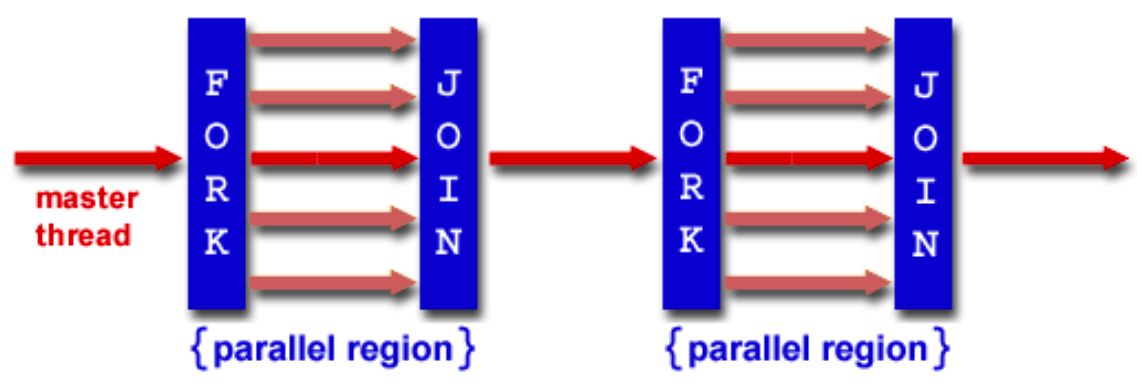
\includegraphics[width=0.7\linewidth]{figures/screenshot064}
\caption{Fork-join parallel execution, used by OpenMP.}
\label{fig:screenshot064}
\end{figure}

All OpenMP programs begin as a single process: the master thread. The master thread executes sequentially until the first parallel region construct is encountered.

The master thread then creates a team of parallel threads; this is the \textit{fork} step.

The statements in the program that are enclosed by the parallel region construct are then executed in parallel among the various team threads.

When the team threads complete the statements in the parallel region construct, they synchronize and terminate, leaving only the master thread; this is the \textit{join} step.

Most OpenMP parallelism is specified through the use of compiler directives which are embedded in C/C++ or Fortran source code. Additionally, there are optional features that implementations are not required to support: \begin{itemize}
\item The API provides for the placement of parallel constructs inside of other parallel constructs - that is, nested parallelism.
\item The API provides for dynamically altering the number of threads which may be used to execute different parallel regions.
\end{itemize}

\subsubsection{I/O}
OpenMP specifies nothing about parallel I/O; this is particularly important if multiple threads attempt to write/read from the same file. If every thread conducts I/O to a different file, the issues are not as significant. It is entirely up to the programmer to ensure that I/O is conducted correctly within the context of a multi-threaded program.

OpenMP provides a \textit{relaxed-consistency} and \textit{temporary} view of thread memory (in their words). In other words, threads can cache their data and are not required to maintain exact consistency with real memory all of the time. When it is critical that all threads view a shared variable identically, the programmer is responsible for ensuring that the variable has been \textit{flushed} by all threads as appropriate (that is, the state of the variable is synchronised with real memory for all threads).

\subsection{Examples}
\autoref{alg:ompexample} demonstrates the use of OpenMP in C. Note how parallelism is delivered by compiler directives (the \texttt{\#pragma}s).
To compile the example, use \texttt{gcc -fopenmp omp\_hello.c -o hello}. To execute the example, use \texttt{./hello} (Linux, Unix, Mac OS X) or \texttt{./hello.exe} (Windows). By default, OpenMP will set the number of threads to equal the number of available CPUs. The number of threads to use can be set by changing the \texttt{OMP\_NUM\_THREADS} environment variable.

\begin{algorithm}[h]
\caption{OpenMP example by Blaise Barney.}
\label{alg:ompexample}
\begin{lstlisting}[language=c]
#include <omp.h>
#include <stdio.h>
#include <stdlib.h>

int main(int argc, char* argv[])
{
    int nthreads, tid;

/* Fork a team of threads giving them their own copies of variables */
#pragma omp parallel private(nthreads, tid) {
    /* Obtain thread number */
    tid = omp_get_thread_num();
    printf("Hello World from thread = %d\n", tid);
    /* Only master thread does this */
    if (tid == 0) {
        nthreads = omp_get_num_threads();
        printf("Number of threads = %d\n", nthreads);
    }
}
/* All threads join master thread and disband */

}
\end{lstlisting}
\end{algorithm}



Your output will look similar to the following; the actual order of output strings may vary:
\begin{lstlisting}
Hello World from thread = 0 
Number of threads = 4 
Hello World from thread = 3 
Hello World from thread = 1 
Hello World from thread = 2  
\end{lstlisting}

\autoref{alg:ompworkshareexample} shows the use of OpenMP for worksharing. Note the use of additional \texttt{\#pragma}s, as well as the use of chunking.

\begin{algorithm}[H]
\caption{OpenMP workshare example by Blaise Barney.}
\label{alg:ompworkshareexample}
\begin{lstlisting}[language=c]
#include <omp.h>
#include <stdio.h>
#include <stdlib.h>
#define CHUNKSIZE 10
#define N 100

int main(int argc, char* argv[])
{
    int nthreads, tid, i, chunk;
    float a[N], b[N], c[N];
    /* Some initializations */
    for (i = 0; i < N; i++)
        a[i] = b[i] = i * 1.0;
    chunk = CHUNKSIZE;

#pragma omp parallel shared(a, b, c, nthreads, chunk) private(i, tid) {
      tid = omp_get_thread_num();
      if (tid == 0) {
          nthreads = omp_get_num_threads();
          printf("Number of threads = %d\n", nthreads);
      }
      printf("Thread %d starting...\n", tid);

      #pragma omp for schedule(dynamic, chunk)
      for (i = 0; i < N; i++) {
          c[i] = a[i] + b[i];
          printf("Thread %d: c[%d]= %f\n", tid, i, c[i]);
      }
  }
  /* end of parallel section */
}
\end{lstlisting}
\end{algorithm}

On a dual-core CPU, this produces output similar to the following:
\begin{lstlisting}
Thread 1 starting... 
Number of threads = 2 
Thread 1: c[0]= 0.000000 
Thread 0 starting... 
Thread 1: c[1]= 2.000000 
Thread 0: c[10]= 20.000000 
Thread 1: c[2]= 4.000000 
Thread 0: c[11]= 22.000000 
Thread 1: c[3]= 6.000000 
Thread 0: c[12]= 24.000000 
Thread 1: c[4]= 8.000000 
Thread 1: c[5]= 10.000000 
...
\end{lstlisting}

\section{GPGPU}
Traditional CPU design is suited to sequential processing. Graphics require data parallelism, which forms the design basis of the \textit{graphics processing unit}, or GPU. The GPU can be extended for use with non-graphic data - \textit{general-purpose GPU}, or \textit{GPGPU} - which allows for very high performance virtually free of cost.

However, only certain types of applications can benefit from this approach. Additionally, GPGPU programming requires the use of special libraries; however, pre-existing software and wrappers are available in some cases.

GPGPU was made possible with the addition of programmable stages and higher precision arithmetic to the rendering pipelines; these pipelines were originally used to facilitate rasterization-based rendering. With this functionality, stream processing on non-graphics data was made possible.

Stream processing is a computing model based on the SIMD paradigm. Some applications can be easily parallelised within the limits of this style of processing; they can utilise the multiple floating point units on the GPU. Allocation, synchronisation and communication, which are usually required in SIMD, are assumed to be automatically managed by the units in this model.

The model simplifies parallel software and hardware by restricting the parallel computation that can be performed. Computation is performed with two components: \begin{itemize}
\item A \textbf{data set} constitutes a (data) stream.
\item A \textbf{kernel function} is a series of operations that is applied to each element in the stream. It is commonly defined as a series of nested loops with no data specification.
\end{itemize}

Several features of the programming model facilitate high-performance programming. \textit{Uniform streaming}, where the same kernel function is applied to all elements in the stream, is common. Kernel functions are typically \textit{pipelined}, and local on-chip memory is reused to minimise external memory bandwidth. As the kernel and stream abstractions expose data dependencies by design, compilers can fully automate and optimise on-chip management tasks to maximise performance.

A kernel requires that stream data abide by two characteristics: being independent and local \footnote{Not explained in the slides}. The kernel defines the basic unit of data for both input and output, allowing the hardware to better allocate resources and schedule I/O; this definition is usually explicit in the kernel, which is expected to have well-defined structures for I/O.

Compute blocks that are well-defined and independent allow scheduling of bulk I/O operations; this scheduling is undertaken in such a way to leverage the underlying hardware cache and memory bus in the most efficient manner possible. Additionally, values associated with a single kernel invocation (that is, values local to that kernel) are treated as local variables and thus use fast kernel-local registers.

Generally, the following type of applications will benefit from stream computing: \begin{itemize}
\item Compute intensive applications where the number of arithmetic operations per each I/O or global memory access operation is large, such that performance is bound by computation and not I/O. 
\item Applications with data parallelism where the same kernel function can be applied to records of an input stream, and a number of records can be processed simultaneously without waiting for results from previous records.
\item Applications with data locality where data is produced once, read once or twice later in the application, and never read again. Intermediate streams passed between kernels, as well as intermediate data within kernel functions, can capture this locality directly using the stream processing programming model.  
\end{itemize}

Notable stream processing languages include the open standards of ACOTES (based on OpenMP) and OpenCL, and the vendor-specific solutions of BROOK+ from AMD and Compute Unified Device Architecture (CUDA) from NVIDIA.

\subsection{OpenCL}
OpenCL is a set of open specifications for a stream processing framework; it is designed for number crunching and parallel computing tasks. Each vendor offers their own implementation, but these implementations must be compliant with the specifications. It was originally proposed with Apple, with NVIDIA and Intel acting as supporting parties.

The specifications were developed by a number of companies, and then handed over to Khronos Group to be maintained. Khronos offer the contents for free without a license free, and are also responsible for maintaining the OpenGL specifications.

OpenCL codifies a shift from clock-speed (based around sequential processing) to multicore processing (parallel programming, data sharing). Its API provides a good framework for utilising the underlying (parallel) hardware in a portable fashion. It aims to abstract over hardware heterogeneity, and offers CPU and GPU support.

Applications for OpenCL include: \begin{itemize}
\item Image, video and audio processing 
\item Gaming, scientific calculations and simulations. It has interoperability with OpenGL for highly visual data representations.
\item Financial modelling 
\item Computationally intensive data-parallel applications 
\end{itemize}

\subsection{Programming Techniques}
There are several programming techniques used for GPGPU processing. These are discussed below.

\subsubsection{Map}
The map operation simply applies the kernel (the user specified function) to every element in the stream. A simple example is multiplying each value in the stream by a constant (e.g. increasing the brightness of an image). It is simple to implement on the GPU.

\subsubsection{Reduce}
Some computations require calculating a smaller stream (possibly a stream of only 1 element) from a larger stream. This is called a reduction of the stream. Generally, a reduction can be accomplished in multiple steps: \begin{itemize}
\item The results from the previous step are used as the input for the current step.
\item The range over which the operation is applied is reduced until only one stream element remains.
\end{itemize}

\subsubsection{Scatter}
The scatter operation is equivalent to \texttt{a[i] = x} in C. The scatter operation is best defined on the vertex processor, as the vertex processor is able to adjust the position of the vertex, which allows the programmer to control where information is deposited on the grid. By comparison, the fragment processor cannot perform a direct scatter operation because the location of each fragment on the grid is fixed at the time of the fragment's creation and cannot be altered by the programmer.

A scatter implementation would first emit both an output value and an output address followed by a gather operation. 

\subsubsection{Gather}
The gather operation is the opposite of the scatter operation; it is equivalent to \texttt{x = a[i]} in C. This is analogous to image processing in the GPU, where the fragment processor is able to read textures in a random-access fashion. A GPGPU can gather information from any grid cell, or multiple grid cells, as need be.

\subsubsection{Filter / Sort}
Stream filtering is essentially a non-uniform reduction. Filtering involves removing items from the stream based on some criteria.

The sort operation transforms an unordered set of elements into an ordered set of elements. The most common implementation on GPUs uses sorting networks. 

\subsubsection{Search}
The search operation allows the programmer to find a particular element within the stream, or possibly find neighbors of a specified element. The GPU is used to run multiple searches in parallel. 
